\graphicspath{{chapters/_resources/}}

\chapter{Journal Clubs}

\section{11- JC Transcriptional Control in Cancer}

Aula e sede: Aula A214 {[}Dipartimenti - POVO{]} Docente: Cusanelli
Emilio Giorno: October 28, 2022 Insegnamento: Transcriptional Control in
Cancer Ora: 10:30 - 12:30 Status: Attended : 11

\hypertarget{myc-recruits-spt5-to-rna-polymerase-ii-to-promote-processive-transcription-elongation}{%
\subsection{MYC Recruits SPT5 to RNA Polymerase II to Promote Processive
Transcription
Elongation}\label{myc-recruits-spt5-to-rna-polymerase-ii-to-promote-processive-transcription-elongation}}

\begin{figure}
\centering
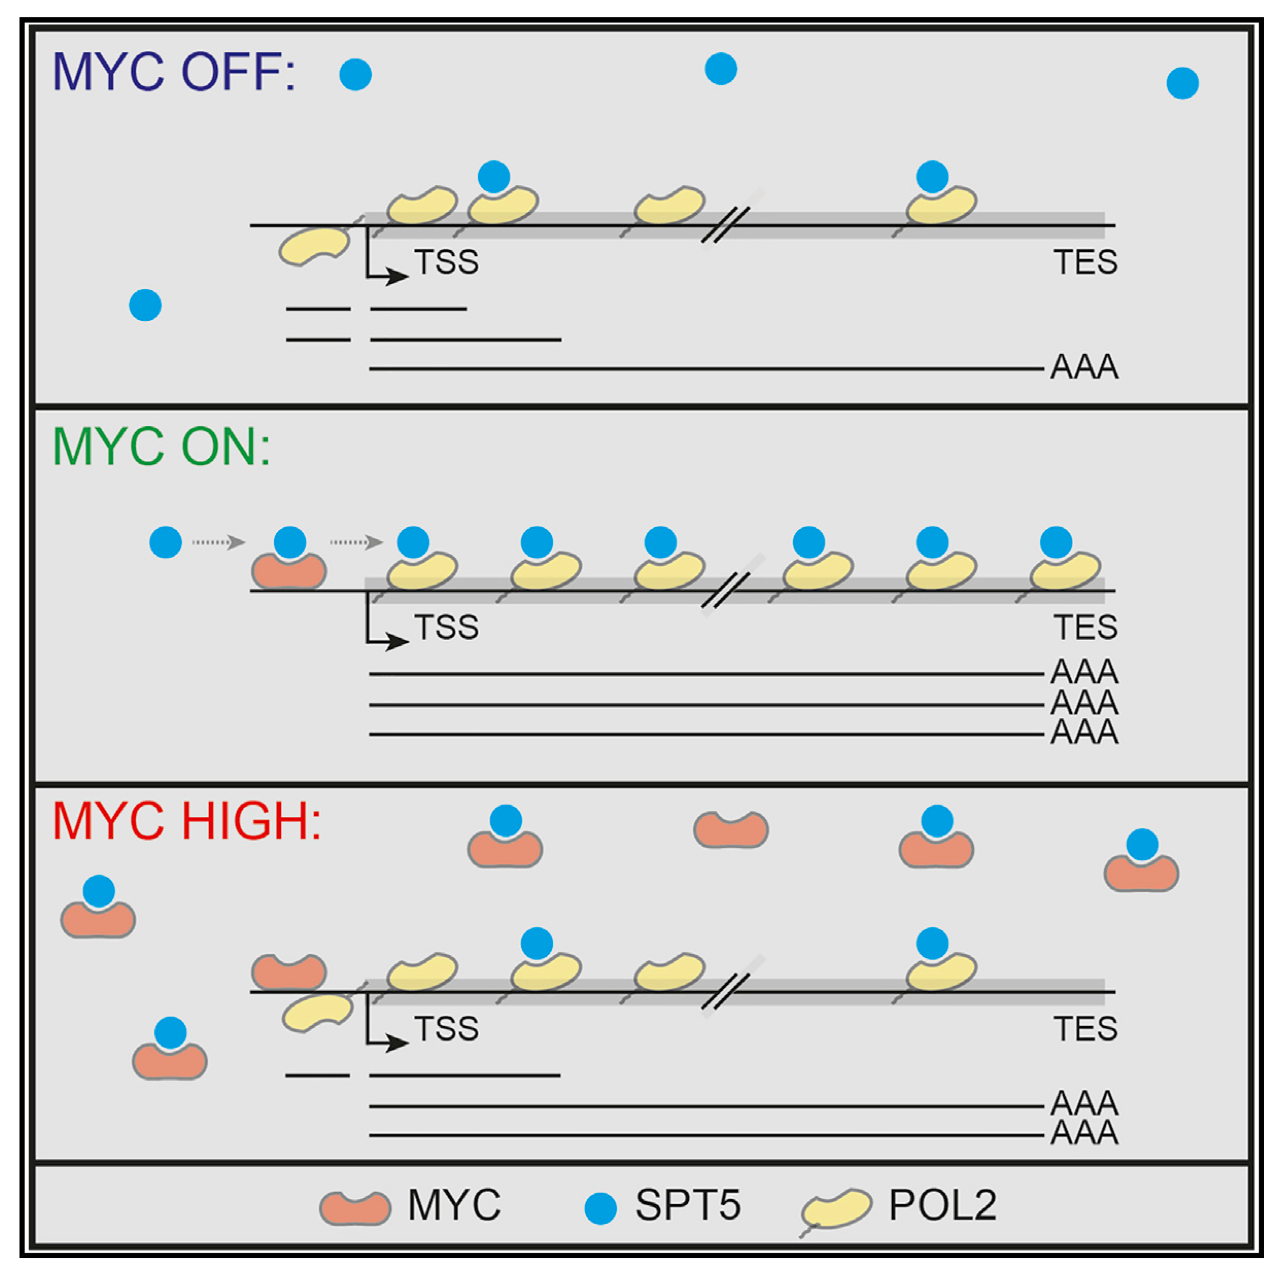
\includegraphics[width=0.5\textwidth]{../_resources/Screenshot_2022-10-28_at_10-37-23.png}
\caption{Screenshot 2022-10-28 at 10.37.23.png}
\end{figure}

MYC is able to modulate the transcriptional cycle, and two mechanism are
proposed:

\begin{itemize}
\tightlist
\item
  MYC can recruit CDK9 to mediate pause release
\item
  MYC transfers Pol II associated factor PAF
\end{itemize}

\hypertarget{tet-offon-transgenic-system}{%
\subsubsection{Tet-Off/On transgenic
system:}\label{tet-offon-transgenic-system}}

A tetracycline-controlled transactivator protein (tTA), which is
composed of the Tet repressor DNA binding protein (TetR) from the Tc
resistance operon of Escherichia coli transposon Tn10 fused to the
strong transactivating domain of VP16 from Herpes simplex virus,
regulates expression of a target gene that is under transcriptional
control of a tetracycline-responsive promoter element (TRE).

Tet-Off expression system: in absence of tetracyclin, tTA binds to the
element leading to active transcription. When we add tetracyclin or Tc
derivatives, the protein is removed from the regulatory element.

In Tet-On we have the opposite scenario.

\hypertarget{myc-controls-the-assembly-of-transcriptionally-engaged-pol-ii-complexes}{%
\subsubsection{MYC Controls the Assembly of Transcriptionally Engaged
Pol II
Complexes}\label{myc-controls-the-assembly-of-transcriptionally-engaged-pol-ii-complexes}}

\begin{itemize}
\tightlist
\item
  6 common proteins in pol II and MYC interactome, but only SPT5 and
  SPT6 changed their association with Pol II upon MYC depletion
\item
  upon MYC depletion, read distribution at all expressed genes showed a
  global reduction of SPT5 binding → chromatin- associated Pol II binds
  to less SPT5 in the absence of MYC
\end{itemize}

\textbf{In situ Proximity Ligation Assay (PLA):} two antibodies with
oligonucleotides which hybridize with a DNA strand, which will only be
able to circularize if sites match. Rolling circle amplification is
performed and ligation is detected.

\begin{itemize}
\tightlist
\item
  Upon MYC depletion we observe less interaction among SPT5 and Pol II
\item
  MYC recruits SPT5 by binding to its N-Terminal region
\end{itemize}

\hypertarget{cdk7-activity-is-required-for-transfer-of-spt5-from-myc-to-pol-ii}{%
\subsubsection{CDK7 Activity is Required for Transfer of SPT5 from MYC
to Pol
II}\label{cdk7-activity-is-required-for-transfer-of-spt5-from-myc-to-pol-ii}}

\begin{itemize}
\tightlist
\item
  MYC facilitates the CDK7-dependent assembly of Pol II-SPT5 complexes.
\end{itemize}

\hypertarget{myc-influences-processivity-and-directionality-of-pol-ii-after-pause-release}{%
\subsubsection{MYC Influences Processivity and Directionality of Pol II
after pause
release}\label{myc-influences-processivity-and-directionality-of-pol-ii-after-pause-release}}

\begin{itemize}
\tightlist
\item
  Reduced processivity and directionality upon MYC depletion
\item
  MYC Maintains High Pol II Elongation Rates
\item
  Overexpression of MYC has an inhibitory effect on Pol II elongation
  rate. SPT4 is sequestered by MYC, and therefore its binding with Pol
  II is decreased. Certain genes lose processivity and directionality at
  oncogenic levels of MYC → MYC dependent sequestration of SPT5 might
  repress tumor-suppressive genes.
\end{itemize}

MYC is not a pioneer TF, it only binds to accessible binding sites. MYC
is able to bind low-affinity binding sites in a scenario of MYC
overexpression.

\hypertarget{brd4-directed-super-enhancer-organization-of-transcription-repression-programs-links-to-chemotherapeutic-efficacy-in-breast-cancer}{%
\subsection{BRD4-directed super-enhancer organization of transcription
repression programs links to chemotherapeutic efficacy in breast
cancer}\label{brd4-directed-super-enhancer-organization-of-transcription-repression-programs-links-to-chemotherapeutic-efficacy-in-breast-cancer}}

BET are epigenetic leaders, they can recognize marks through
bromodomain. \textbf{BRD4} is a positive regulator of transcription. It
is involved in some disorders, as inflammation, obesity and cancer, as
it can enhance the transcription of oncogenes. JQ1 inhibits BET4 and is
a promising antitumor drug, but a resistance can be developed.

\textbf{Super-enhancers} are clusters of enhancers occupied by master
regulators e.g.~BRD4 or Mediator, which control the expression of
lineage-specific genes.

\begin{itemize}
\tightlist
\item
  NuRD complex: multi-subunit, repressor. Acts as chromatin remodeling
  complex and histone deacetylase.
\item
  LSD1: histone demethylase
\item
  Pellino (PEL1): E3 ubiquitin ligase
\end{itemize}

\hypertarget{brd4-is-physically-associated-with-lsd1nurd-complex}{%
\subsubsection{BRD4 is physically associated with LSD1/NuRD
complex}\label{brd4-is-physically-associated-with-lsd1nurd-complex}}

Immunoaffinity purification + MS: FLAG tagged BRD4, isolate through
magnetic beads. IP, elution and silver staining. Thanks to MF we can
identify interactors: all the components of LSD1/NuRD complex, confirmed
by Western Blotting and coIP assays.

BRD4 is directly interacting with LSD1 through the C-terminus

\hypertarget{brd4-and-the-lsd1nurd-complex-occupy-se}{%
\subsubsection{BRD4 and the LSD1/NuRD complex occupy
SE}\label{brd4-and-the-lsd1nurd-complex-occupy-se}}

Interaction with factors known to reside in super-enhancer regions
e.g.~MED-1. Consolidated with ChIP-seq, almost 23000 targets in common.
The sequences bound are enriched in H3Kme1 and H3k27ac.

SE control genes in important signalling pathways and drug resistance
e.g.~PDPK1

\hypertarget{decommissioning-the-brd4lsd1nurd-complex-leads-to-jq1-resistance}{%
\subsubsection{Decommissioning the BRD4/LSD1/NuRD Complex Leads to JQ1
Resistance}\label{decommissioning-the-brd4lsd1nurd-complex-leads-to-jq1-resistance}}

After 4 weeks cancer resistant cells emerge. BRD4 is quickly inhibited,
while LSD1 or MTA3 in the early phase of treatment maintain chromatin
contact, which is exactly lost at 4 weeks.

\begin{enumerate}
\def\labelenumi{\arabic{enumi}.}
\tightlist
\item
  removal of LSD1
\item
  increase of target genes expression
\item
  emergence of drug resistance
\end{enumerate}

BRD4 is required for LSD1/NuRD recruitment at super-enhancers

Reduced occupancy could be due to the lower protein levels: LSD1 mRNA
expression level is table upon JQ1 inhibition, but protein levels are
lower → proteosome action degrades the protein.

\hypertarget{elimination-of-peli1-improves-the-therapeutic-efficacy-of-jq1-in-breast-cancer-cells}{%
\subsubsection{Elimination of PELI1 Improves the Therapeutic Efficacy of
JQ1 in Breast Cancer
Cells}\label{elimination-of-peli1-improves-the-therapeutic-efficacy-of-jq1-in-breast-cancer-cells}}

\begin{itemize}
\tightlist
\item
  Of 6 E3 ligases candidates, only PELI1 knockdown results in a strong
  increase of LSD1
\item
  PELI1 inhibition improves JQ1 therapeutic efficacy
\item
  the removal of BRD4/LSD1/NuRD complex from chromatin allows cancer
  cells to evade the selective pressure induced by JQ1 or other anti
  tumor drugs.
\end{itemize}

\hypertarget{the-clinicopathological-significance-of-the-peli1-lsd1-brd4lsd1-nurd-axis-in-breast-cancer}{%
\subsubsection{The Clinicopathological Significance of the
PELI1-LSD1-BRD4/LSD1/ NuRD Axis in Breast
Cancer}\label{the-clinicopathological-significance-of-the-peli1-lsd1-brd4lsd1-nurd-axis-in-breast-cancer}}

\begin{itemize}
\tightlist
\item
  PELI1 mRNA levels are up-regulated when at least chemotherapy are
  applied
\item
  high expression of PELI1 leads to a worse survival rate
\end{itemize}

\begin{figure}
\centering
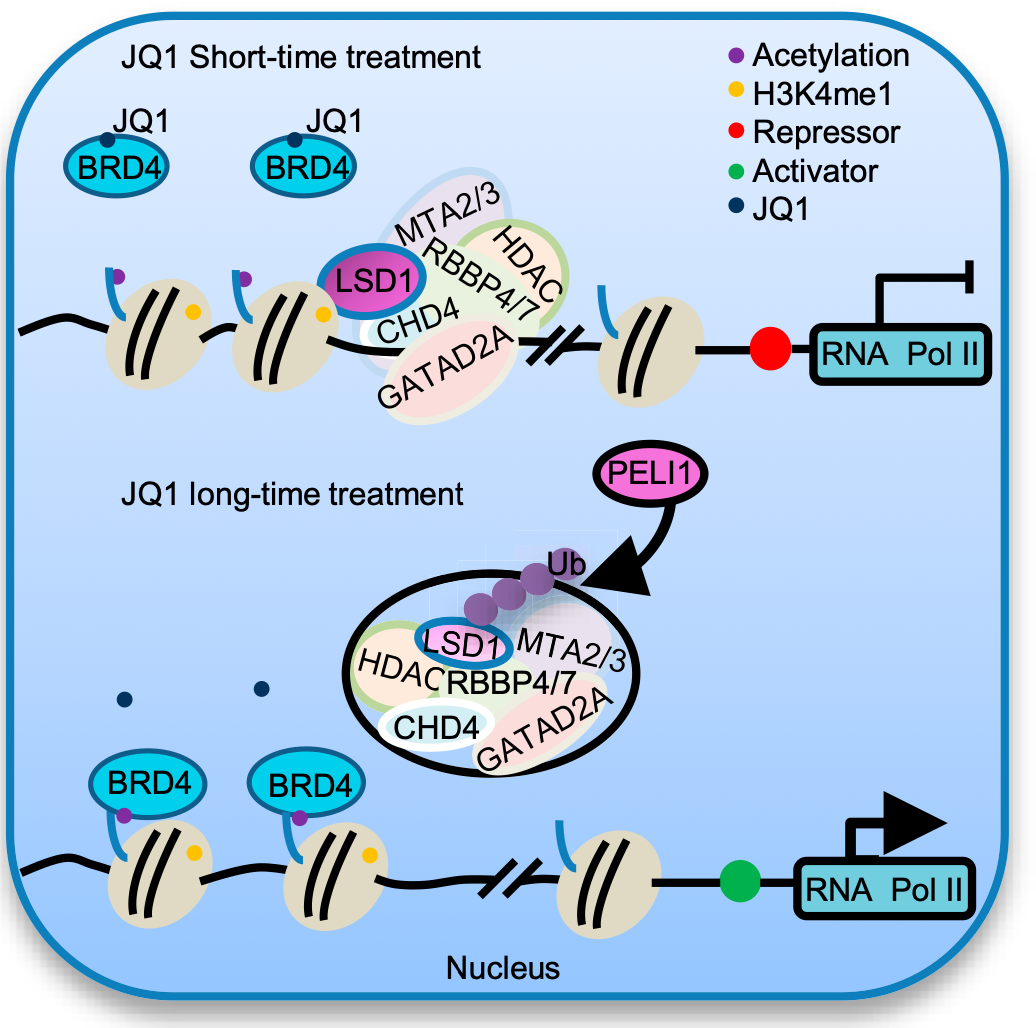
\includegraphics[width=0.5\textwidth]{../_resources/Screenshot_2022-10-28_at_11-55-04.png}
\caption{Screenshot 2022-10-28 at 11.55.04.png}
\end{figure}

Proposal: combined targeting of BRD4 and PELI1 as therapeutic for breast
cancer
